\documentclass[conference]{IEEEtran}
\IEEEoverridecommandlockouts
% The preceding line is only needed to identify funding in the first footnote. If that is unneeded, please comment it out.
\usepackage{cite}
\usepackage{amsmath,amssymb,amsfonts}
\usepackage{algorithmic}
\usepackage{graphicx}
\usepackage{textcomp}
\usepackage{xcolor}
\def\BibTeX{{\rm B\kern-.05em{\sc i\kern-.025em b}\kern-.08em
    T\kern-.1667em\lower.7ex\hbox{E}\kern-.125emX}}
\begin{document}

\title{A Software System for maintaining Attendance\\
}

\author{\IEEEauthorblockN{Rudransh Pratap Singh}
\IEEEauthorblockA{{\textbf{IIIT-H}} \\
Gachibowli, Hyderabad \\
rudransh.s@research.iiit.ac.in}

}

\maketitle

\begin{abstract}
Recording Attendance has been a major issue, with most current systems vulnerable to proxies. The paper proposes a novel software system
based on computer vision methods such as face recognition to detect and record attendance. The system is designed to be robust and scalable.
\end{abstract}

\section{Introduction}
The COVID - 19 pandemic has deferred the offline mode of classrooms for quite some time now, but now that everything seems to go back to normal, issues that were once forgotten are now coming up again. One of such issues is recording the attendance of students.
\par 
The current method of recording attendance is as follows. Students are assigned designated seats for their respective classes. A designated person comes up with a register, marks the empty seats, and marks the 
students corresponding to those seats as \textbf{absent}. This, however, is an extremely inefficient method, primarily because of the following reasons.
\begin{enumerate}
    \item The procedure is entirely manual, and hence it will take a lot of effort and time to figure out the empty seats and mark the students absent. This problem is especially aggravated in the case of large classes, which span over a huge area, with lots of students.
    \item This method is extremely vulnerable to proxies; students can ask other students, who might not have the course, to take their seats. Since the registrar has no idea of what the actual person looks. They are bound to mark the person as present, this is done in practice, and hence the system is vulnerable to proxies.
    \item The student does not need to be available throughout the class and can sneak in for attendance when the registrar comes in. The registrar has no idea when the student joined or left the class.
    \item The system is heavily reliant on trusting the moral character of the registrar. A student can bribe the registrar to mark the student as present, for the entirety of the course.
\end{enumerate}
Also, we consider that the registrar is completely accurate in their work, which is not true. There might be students present in class who might have been accidentally 
marked absent by the registrar because of human error. All of these mean one thing: the current recording attendance system needs to change.
\par
This is where we come up with a novel method to record attendance. The system is based on computer vision methods, such as face recognition, to detect and record attendance. The system is designed to be scalable, as well as transparent to the students themselves, that is in case of any errors, the student can dispute the attendance.


\section{Literature Review}
A lot of research has been done on methods for recording attendance, and several methods have been proposed for the same. We look at a few of them in this section.
\subsection*{A. RFID Authentication}
One of the more common approaches to solving the attendance problem is by means of Radio Frequency Identification (RFID) tags. RFID tags are a type of tag that can be placed on any object, such as an ID-card, and can be read by a reader. The reader can then read the tag and determine if the person is present or absent.
RFID has a wide variety of applications other than just attendance. As of now, IIITH aims to use RFID tags for recording mess attendance. The only issue with this method is that there is no way to automatically verify the actual owner of the RFID tag, and as a result, one could proxy the attendance of a student by using their RFID-tagged cards.
\subsection*{B. Biometric Authentication}
Another approach to solving this problem is through the use of biometrics, wherein one uses their fingerprints for identification and authentication. \\ \\
Since our approach is primarily through the means of face recognition, therefore some of the ongoing research in the field currently under investigation are as follows 

\subsection*{C. YOLO : You Only Look Once}
Most object detection algorithm are essentially classifiers, which assign a given data point to one of many classes. 
However YOLO instead treats this as a regression problem to spatially separated bounding boxes and associated class probablities.. Then when a test image is provided, it predicts the bounding boxes and class probablities for each object in the image.
\par 
One of the main advantages of YOLO is it's speed, the base model can process images in real-time at around 45 frames per second. Another variant of YOLO, called the Fast-YOLO can process images at 155 frames per second, while achieving double the mAP(mean average precision) of other real-time object detection algorithms.

\subsection*{D. FaceNet}
While there have been significant developments in the field of face recognition, implementing such algorithms at large scale is still a huge task. This brings in FaceNet, which basically learns the mapping from different face images to an Euclidean space, with metric distances associated between any two faces.
One could then run the standard clustering/classification/regression algorithms on this mapped dataset, using FaceNet embeddings as feature vectors. The mapping is extremely accurate, when tested on the LFW (Labelled Faces in the Wild) dataset, it achieved a record breaking accuracy of 99.6\%, and an accuracy of 95.12\% on the YouTube Faces database.
\section{System Architecture}
The system architecture is perhaps the most important part of developing any software system, since 
it essentially describes the way to tackle the aforementioned problem. This will be extremely useful for software developers during the early stages of the development. In this section
we provide the basic description of the system, mentioning the requirements, the use cases, as well as providing Use Case diagrams, sequence diagrams, and class diagrams for the entire structure as well.
\subsection[]{Requirements}
In order to provide facial recognition support for classes, we must have some means to capture the faces during the class. We do this by means of a high-resolution camera, which is able to capture detail at a very fine level. 
This will be extremely important, since our system requires monitoring of students in the class, where the sizes of the class can be extremely large.
We install two of these cameras per class, one of which shall be placed near the entrance, and the other shall be placed at inside the class, at a location with clear lighting, and little to no obstruction.
\par
We shall also need to take care of storage. For the purposes of the system, which shall be described later, we require the recordings of the camera as well, atleast for a duration of one day. Therefore a separate storage server needs to be implemented.
\begin{enumerate}
    \item Functional Requirements : The user should be able to login to the application using CAS authentication; The user must be able to see whether his attendance was recorded or not; the user should be able to raise a ticket in case of disputes.
    \item Non Functional Requirements : Reliablity, Robustness, and Scalability are the primary non functional requirements for this software system. The Face recognition and identifier must be able to perform real time computations, interoperablity across different computer systems as well as mobile devices, along with a modular system, and a flexible interface for ease of integration
\end{enumerate}
\subsection[]{Users}
The system will have primarily three users :
\begin{enumerate}
    \item The registrar/admin, who maintains the recordings, and resolves disputes, if any.
    \item The teacher, who also has access to attendance records of the entire class for his particular course, and can use it to further improve the course structure.
    \item The student, who has access to his own attendance records, for all course assigned to them.
\end{enumerate}
\subsection{Use Cases}
The use cases for each individual user are as follows :
\begin{enumerate}
    \item Student :
        \begin{itemize}
            \item Record attendance of the student.
            \item View attendance of the student.
            \item Find statistics such as most and least atended classes, classes which have attendance lower than limit etc.
            \item raise a ticket in case of any dispute over attendance of a particular course.
        \end{itemize}
    \item Teacher :
        \begin{itemize}
            \item View attendance of the entire class.
            \item View most frequently and least frequently absent students.
        \end{itemize}
    \item Registrar :
        \begin{itemize}
            \item resolve disputes regarding students.
            \item view recordings of class, including recordings from the cameras at the entrance and inside the class itself.
        \end{itemize}
\end{enumerate}
The Primary idea is as follows : The faces of all students are already stored in a pre-existing database, one could use the images present on the ID cards, or create better higher definition ones instead as well. Once a student enters
a class, their faces are captured and run against the database, and once a match is found, their attendance is recorded. This is then followed by a notification, sent as soon as possible to the student. While the student is inside the class, the in-class camera captures his face, and as long as he is visible to the
camera, his attendance score ( a measure between 0 to 100) increases. The attendance score of the student is calculated as follows
\begin{equation}
    attendance\_score=\frac{total\_time\_present}{duratio\_of\_class}
\end{equation}
where \textit{total\_time\_present} is the total time spent by the student in the class, and \textit{duratio\_of\_class} is the duration of the class.
\par
If the student leaves the class at any point in time, the system will automatically stop incrementing his attendance score. It will also notify the student that he has left the class. The student will be marked as present, if his \textit{attendance\_score} is above a certain limit of the class.
\par
If, in case the student was in fact, present, but for some reason, was not detected by the cameras. He/she can raise a ticket to the admin, stating that he was present in the class. The registrar can then 
perform a manual inspection of the recording, checking whether the student at the seat was actually present. If it is indeed the case, the dispute ends with student being marked as present, otherwise 
he will be marked as absent. The ticket can only be raised by the student within 24 hours of the class, since after that the recordings will be purged.
\par
As for the teachers, they have access to the the entire class attendance statistics, and can use information such as the number of people who attended the class, to perhaps gain insight into what his class might be lacking, what he needs
to change in his course structure etc. Also information such as most and least frequently absent students, can be used by the teacher to take one-on-one sessions with these students, understanding why he/she might not like the course etc.
\begin{figure}[h]
    \centering
    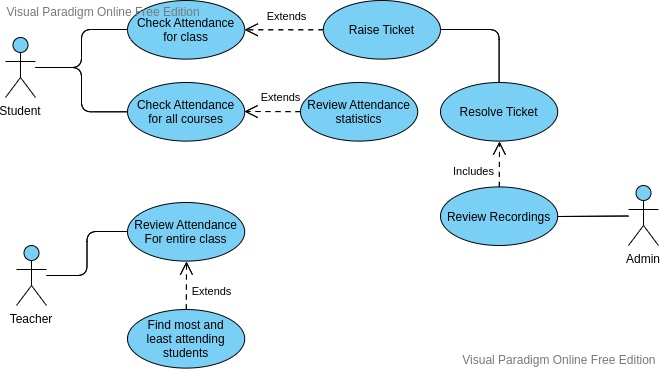
\includegraphics[height=7.5cm,width=9cm]{images/FacialRecogUseCase.png}
    \caption{Use Case Diagram}
    \label{fig:my_label}
\end{figure}

\end{document}
